% Options for packages loaded elsewhere
\PassOptionsToPackage{unicode}{hyperref}
\PassOptionsToPackage{hyphens}{url}
%
\documentclass[
  ignorenonframetext,
  aspectratio=169,
  russian,
]{beamer}
\usepackage{pgfpages}
\setbeamertemplate{caption}[numbered]
\setbeamertemplate{caption label separator}{: }
\setbeamercolor{caption name}{fg=normal text.fg}
\beamertemplatenavigationsymbolsempty
% Prevent slide breaks in the middle of a paragraph
\widowpenalties 1 10000
\raggedbottom
\setbeamertemplate{part page}{
  \centering
  \begin{beamercolorbox}[sep=16pt,center]{part title}
    \usebeamerfont{part title}\insertpart\par
  \end{beamercolorbox}
}
\setbeamertemplate{section page}{
  \centering
  \begin{beamercolorbox}[sep=12pt,center]{section title}
    \usebeamerfont{section title}\insertsection\par
  \end{beamercolorbox}
}
\setbeamertemplate{subsection page}{
  \centering
  \begin{beamercolorbox}[sep=8pt,center]{subsection title}
    \usebeamerfont{subsection title}\insertsubsection\par
  \end{beamercolorbox}
}
\AtBeginPart{
  \frame{\partpage}
}
\AtBeginSection{
  \ifbibliography
  \else
    \frame{\sectionpage}
  \fi
}
\AtBeginSubsection{
  \frame{\subsectionpage}
}

\usepackage{amsmath,amssymb}
\usepackage{iftex}
\ifPDFTeX
  \usepackage[T1]{fontenc}
  \usepackage[utf8]{inputenc}
  \usepackage{textcomp} % provide euro and other symbols
\else % if luatex or xetex
  \usepackage{unicode-math}
  \defaultfontfeatures{Scale=MatchLowercase}
  \defaultfontfeatures[\rmfamily]{Ligatures=TeX,Scale=1}
\fi
\usepackage{lmodern}
\ifPDFTeX\else  
    % xetex/luatex font selection
\fi
% Use upquote if available, for straight quotes in verbatim environments
\IfFileExists{upquote.sty}{\usepackage{upquote}}{}
\IfFileExists{microtype.sty}{% use microtype if available
  \usepackage[]{microtype}
  \UseMicrotypeSet[protrusion]{basicmath} % disable protrusion for tt fonts
}{}
\makeatletter
\@ifundefined{KOMAClassName}{% if non-KOMA class
  \IfFileExists{parskip.sty}{%
    \usepackage{parskip}
  }{% else
    \setlength{\parindent}{0pt}
    \setlength{\parskip}{6pt plus 2pt minus 1pt}}
}{% if KOMA class
  \KOMAoptions{parskip=half}}
\makeatother
\usepackage{xcolor}
\newif\ifbibliography
\setlength{\emergencystretch}{3em} % prevent overfull lines
\setcounter{secnumdepth}{-\maxdimen} % remove section numbering


\providecommand{\tightlist}{%
  \setlength{\itemsep}{0pt}\setlength{\parskip}{0pt}}\usepackage{longtable,booktabs,array}
\usepackage{calc} % for calculating minipage widths
\usepackage{caption}
% Make caption package work with longtable
\makeatletter
\def\fnum@table{\tablename~\thetable}
\makeatother
\usepackage{graphicx}
\makeatletter
\newsavebox\pandoc@box
\newcommand*\pandocbounded[1]{% scales image to fit in text height/width
  \sbox\pandoc@box{#1}%
  \Gscale@div\@tempa{\textheight}{\dimexpr\ht\pandoc@box+\dp\pandoc@box\relax}%
  \Gscale@div\@tempb{\linewidth}{\wd\pandoc@box}%
  \ifdim\@tempb\p@<\@tempa\p@\let\@tempa\@tempb\fi% select the smaller of both
  \ifdim\@tempa\p@<\p@\scalebox{\@tempa}{\usebox\pandoc@box}%
  \else\usebox{\pandoc@box}%
  \fi%
}
% Set default figure placement to htbp
\def\fps@figure{htbp}
\makeatother

\usepackage{polyglossia}
\setmainlanguage{russian}
\setotherlanguage{english}
\usepackage{fontspec}
\setmainfont{FreeSerif}
\setsansfont{FreeSans}
\setmonofont{FreeMono}
\makeatletter
\@ifpackageloaded{caption}{}{\usepackage{caption}}
\AtBeginDocument{%
\ifdefined\contentsname
  \renewcommand*\contentsname{Содержание}
\else
  \newcommand\contentsname{Содержание}
\fi
\ifdefined\listfigurename
  \renewcommand*\listfigurename{Список Иллюстраций}
\else
  \newcommand\listfigurename{Список Иллюстраций}
\fi
\ifdefined\listtablename
  \renewcommand*\listtablename{Список Таблиц}
\else
  \newcommand\listtablename{Список Таблиц}
\fi
\ifdefined\figurename
  \renewcommand*\figurename{Рисунок}
\else
  \newcommand\figurename{Рисунок}
\fi
\ifdefined\tablename
  \renewcommand*\tablename{Таблица}
\else
  \newcommand\tablename{Таблица}
\fi
}
\@ifpackageloaded{float}{}{\usepackage{float}}
\floatstyle{ruled}
\@ifundefined{c@chapter}{\newfloat{codelisting}{h}{lop}}{\newfloat{codelisting}{h}{lop}[chapter]}
\floatname{codelisting}{Список}
\newcommand*\listoflistings{\listof{codelisting}{Список Каталогов}}
\makeatother
\makeatletter
\makeatother
\makeatletter
\@ifpackageloaded{caption}{}{\usepackage{caption}}
\@ifpackageloaded{subcaption}{}{\usepackage{subcaption}}
\makeatother

\ifLuaTeX
\usepackage[bidi=basic]{babel}
\else
\usepackage[bidi=default]{babel}
\fi
\babelprovide[main,import]{russian}
% get rid of language-specific shorthands (see #6817):
\let\LanguageShortHands\languageshorthands
\def\languageshorthands#1{}
\usepackage{csquotes}
\usepackage{bookmark}

\IfFileExists{xurl.sty}{\usepackage{xurl}}{} % add URL line breaks if available
\urlstyle{same} % disable monospaced font for URLs
\hypersetup{
  pdftitle={Презентация по лабораторной работе 3},
  pdfauthor={Курилко-Рюмин Евгений Михайлович},
  pdflang={ru},
  hidelinks,
  pdfcreator={LaTeX via pandoc}}


\title{Презентация по лабораторной работе 3}
\subtitle{Агентное Моделирование}
\author{Курилко-Рюмин Евгений Михайлович}
\date{2026-03-21}

\begin{document}
\frame{\titlepage}

\renewcommand*\contentsname{Содержание}
\begin{frame}[allowframebreaks]
  \frametitle{Содержание}
  \setcounter{tocdepth}{3}
  \tableofcontents
\end{frame}

\section{Информация}\label{ux438ux43dux444ux43eux440ux43cux430ux446ux438ux44f}

\begin{frame}{Докладчик}
\phantomsection\label{ux434ux43eux43aux43bux430ux434ux447ux438ux43a}
\begin{columns}[c]
\begin{column}{0.7\linewidth}
\begin{itemize}
\tightlist
\item
  Курилко-Рюмин Евгений Михайлович
\item
  Студент
\item
  Российский университет дружбы народов им. П. Лумумбы
\item
  \href{mailto:1132232883@rudn.ru}{\nolinkurl{1132232883@rudn.ru}}
\item
  \url{https://emkurilkoryumin.github.io/ru/}
\end{itemize}
\end{column}
\end{columns}
\end{frame}

\section{Цель и
задачи}\label{ux446ux435ux43bux44c-ux438-ux437ux430ux434ux430ux447ux438}

\begin{frame}{Цель работы}
\phantomsection\label{ux446ux435ux43bux44c-ux440ux430ux431ux43eux442ux44b}
\begin{itemize}
\tightlist
\item
  Изучить принципы агентного моделирования (ABM)
\item
  Реализовать модель Daisyworld с помощью Agents.jl
\item
  Исследовать механизмы саморегуляции климата
\item
  Применить литературное программирование (Literate.jl)
\end{itemize}
\end{frame}

\begin{frame}{Задание}
\phantomsection\label{ux437ux430ux434ux430ux43dux438ux435}
\begin{enumerate}
\tightlist
\item
  Создать проект DrWatson, установить пакеты
\item
  Реализовать модель Daisyworld (7 скриптов)
\item
  Для каждого скрипта: литературная версия, генерация 3 форматов
\item
  Провести параметрическое исследование
\item
  Интегрировать результаты в отчёт
\end{enumerate}
\end{frame}

\section{Теоретическое
введение}\label{ux442ux435ux43eux440ux435ux442ux438ux447ux435ux441ux43aux43eux435-ux432ux432ux435ux434ux435ux43dux438ux435}

\begin{frame}{Агентное моделирование (ABM)}
\phantomsection\label{ux430ux433ux435ux43dux442ux43dux43eux435-ux43cux43eux434ux435ux43bux438ux440ux43eux432ux430ux43dux438ux435-abm}
\begin{itemize}
\tightlist
\item
  \textbf{Агент} --- автономная сущность с правилами поведения
\item
  \textbf{Среда} --- пространство взаимодействия (сетка
  \(30 \times 30\))
\item
  \textbf{Эмерджентность} --- глобальное поведение из локальных правил
\item
  \textbf{Гетерогенность} --- агенты различаются по свойствам
\item
  Инструмент: фреймворк \textbf{Agents.jl} для Julia
\end{itemize}
\end{frame}

\begin{frame}{Модель Daisyworld}
\phantomsection\label{ux43cux43eux434ux435ux43bux44c-daisyworld}
\begin{itemize}
\tightlist
\item
  Предложена Лавлоком и Уотсоном (1983), гипотеза Геи
\item
  Два вида маргариток: чёрные (\(\alpha = 0.25\)) и белые
  (\(\alpha = 0.75\))
\item
  Формула нагрева: \(T = 72 \ln((1-\alpha) \cdot L) + 80\)
\item
  Порог размножения: \(p = 0.1457T - 0.0032T^2 - 0.6443\)
\end{itemize}
\end{frame}

\section{Настройка
окружения}\label{ux43dux430ux441ux442ux440ux43eux439ux43aux430-ux43eux43aux440ux443ux436ux435ux43dux438ux44f}

\begin{frame}{Запуск Julia}
\phantomsection\label{ux437ux430ux43fux443ux441ux43a-julia}
Запуск Julia REPL


\includegraphics[width=0.6\linewidth,height=\textheight,keepaspectratio]{../report/image/1.png}
\end{frame}

\begin{frame}{Загрузка DrWatson}
\phantomsection\label{ux437ux430ux433ux440ux443ux437ux43aux430-drwatson}
Подключение пакета DrWatson


\includegraphics[width=0.6\linewidth,height=\textheight,keepaspectratio]{../report/image/2.png}
\end{frame}

\begin{frame}{Создание проекта DrWatson}
\phantomsection\label{ux441ux43eux437ux434ux430ux43dux438ux435-ux43fux440ux43eux435ux43aux442ux430-drwatson}
Инициализация проекта


\includegraphics[width=0.6\linewidth,height=\textheight,keepaspectratio]{../report/image/2.png}
\end{frame}

\begin{frame}{Установка пакетов}
\phantomsection\label{ux443ux441ux442ux430ux43dux43eux432ux43aux430-ux43fux430ux43aux435ux442ux43eux432}
Добавление Julia-пакетов


\includegraphics[width=0.6\linewidth,height=\textheight,keepaspectratio]{../report/image/3.png}
\end{frame}

\begin{frame}{Пакеты установлены}
\phantomsection\label{ux43fux430ux43aux435ux442ux44b-ux443ux441ux442ux430ux43dux43eux432ux43bux435ux43dux44b}
Успешная установка пакетов


\includegraphics[width=0.6\linewidth,height=\textheight,keepaspectratio]{../report/image/3.png}
\end{frame}

\section{Базовая
визуализация}\label{ux431ux430ux437ux43eux432ux430ux44f-ux432ux438ux437ux443ux430ux43bux438ux437ux430ux446ux438ux44f}

\begin{frame}{Запуск daisyworld.jl}
\phantomsection\label{ux437ux430ux43fux443ux441ux43a-daisyworld.jl}
Запуск скрипта базовой визуализации


\includegraphics[width=0.6\linewidth,height=\textheight,keepaspectratio]{../report/image/7.png}
\end{frame}

\begin{frame}{Тепловая карта: шаг 0}
\phantomsection\label{ux442ux435ux43fux43bux43eux432ux430ux44f-ux43aux430ux440ux442ux430-ux448ux430ux433-0}
Начальное состояние: 20\% чёрных + 20\% белых

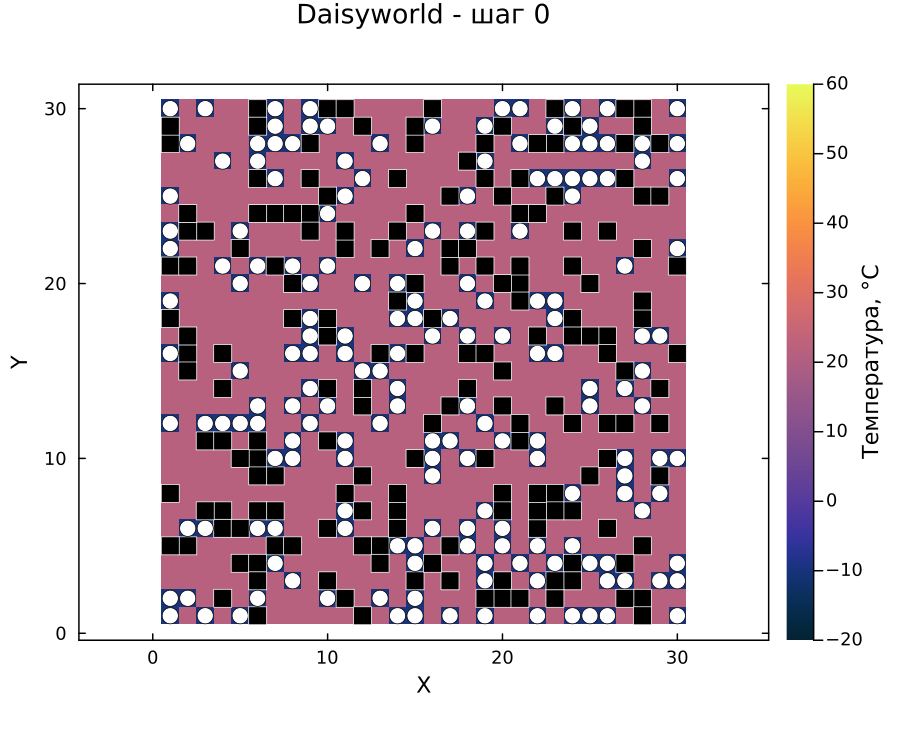
\includegraphics[width=0.5\linewidth,height=\textheight,keepaspectratio]{../report/image/daisyworld_step000.png}
\end{frame}

\begin{frame}{Тепловая карта: шаг 5}
\phantomsection\label{ux442ux435ux43fux43bux43eux432ux430ux44f-ux43aux430ux440ux442ux430-ux448ux430ux433-5}
Маргаритки образуют кластеры

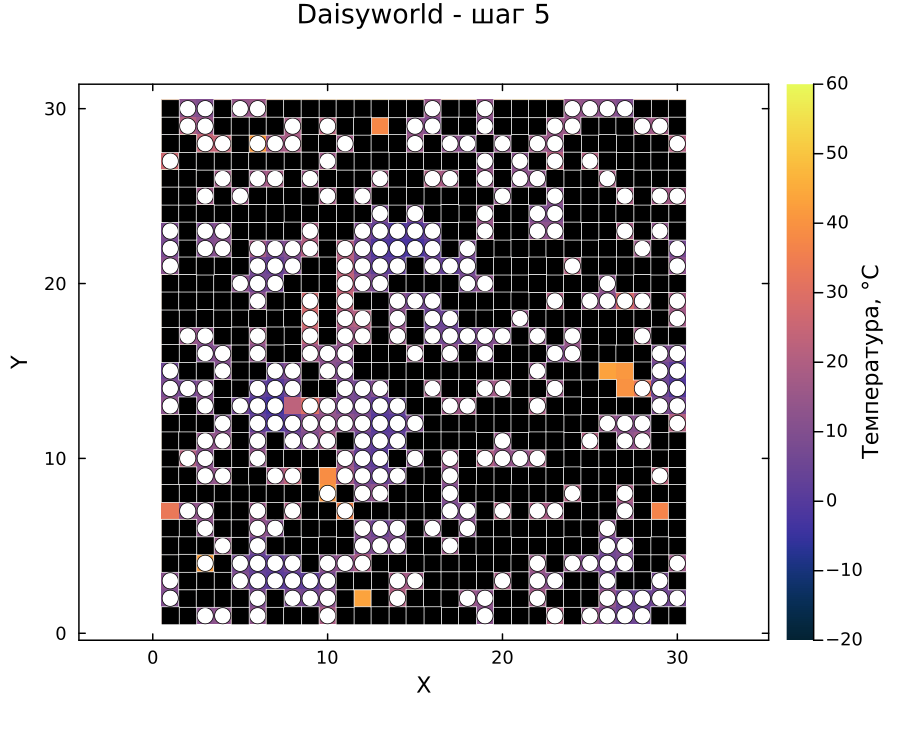
\includegraphics[width=0.5\linewidth,height=\textheight,keepaspectratio]{../report/image/daisyworld_step005.png}
\end{frame}

\begin{frame}{Тепловая карта: шаг 40}
\phantomsection\label{ux442ux435ux43fux43bux43eux432ux430ux44f-ux43aux430ux440ux442ux430-ux448ux430ux433-40}
Динамическое равновесие

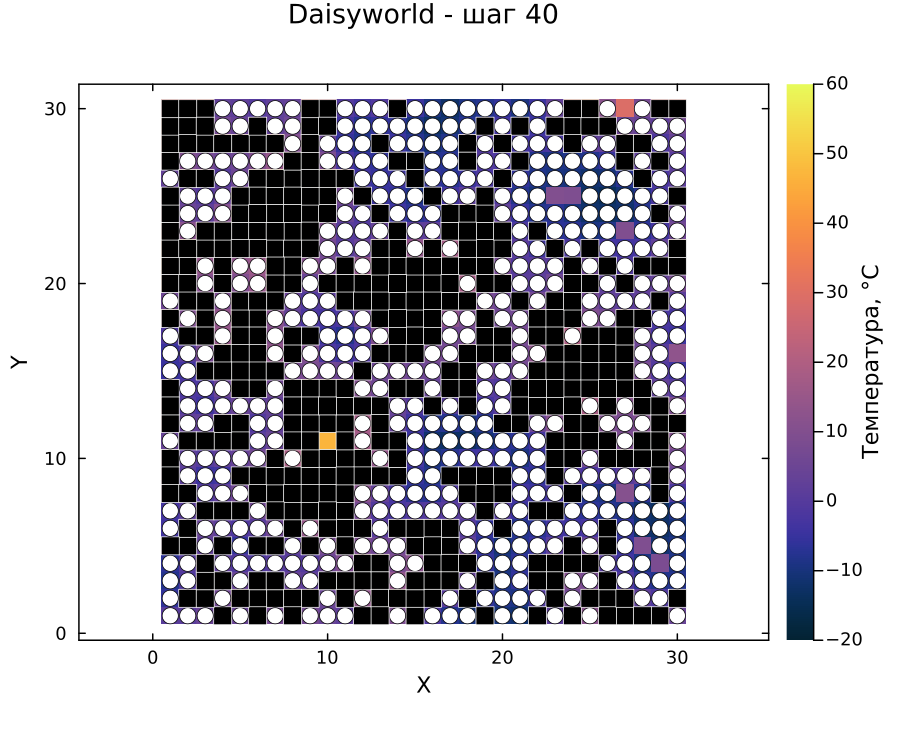
\includegraphics[width=0.5\linewidth,height=\textheight,keepaspectratio]{../report/image/daisyworld_step040.png}
\end{frame}

\begin{frame}{Цикл литературного программирования daisyworld}
\phantomsection\label{ux446ux438ux43aux43b-ux43bux438ux442ux435ux440ux430ux442ux443ux440ux43dux43eux433ux43e-ux43fux440ux43eux433ux440ux430ux43cux43cux438ux440ux43eux432ux430ux43dux438ux44f-daisyworld}
сгенерированы три производных формата


\includegraphics[width=0.6\linewidth,height=\textheight,keepaspectratio]{../report/image/4.png}
\end{frame}

\section{Анимация}\label{ux430ux43dux438ux43cux430ux446ux438ux44f}

\begin{frame}{Запуск анимации}
\phantomsection\label{ux437ux430ux43fux443ux441ux43a-ux430ux43dux438ux43cux430ux446ux438ux438}
Запуск скрипта daisyworld-animate.jl

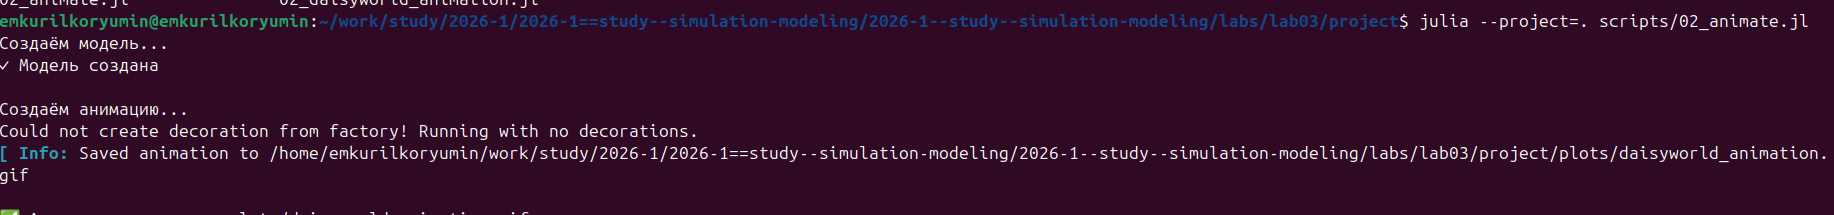
\includegraphics[width=0.6\linewidth,height=\textheight,keepaspectratio]{../report/image/01.png}
\end{frame}

\begin{frame}{Результат анимации}
\phantomsection\label{ux440ux435ux437ux443ux43bux44cux442ux430ux442-ux430ux43dux438ux43cux430ux446ux438ux438}
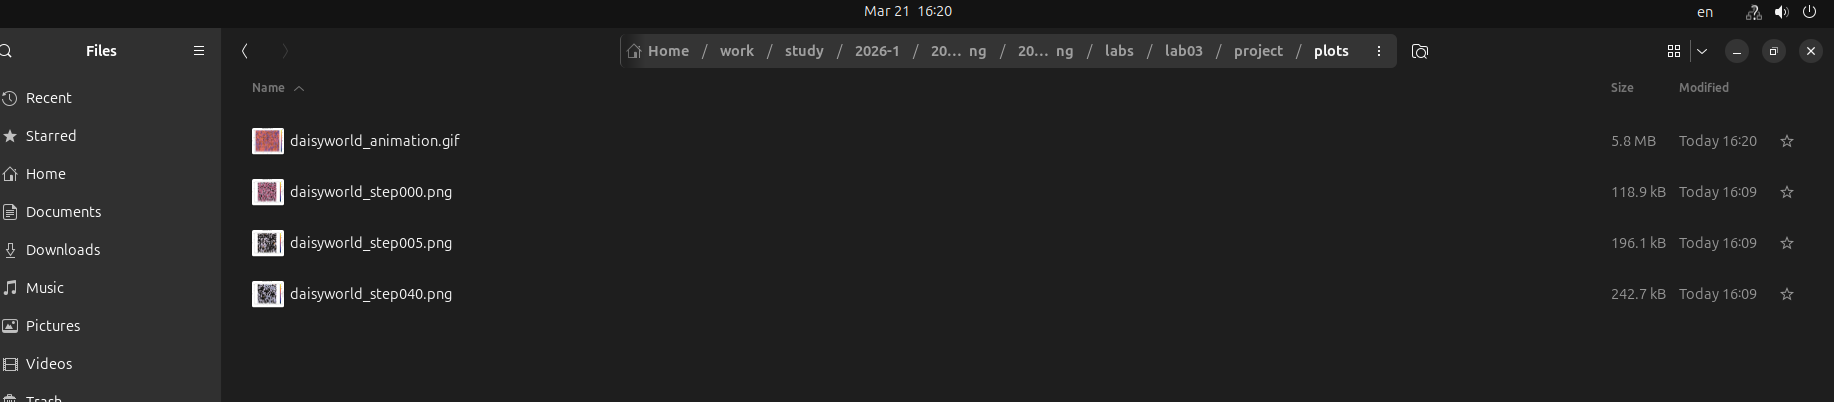
\includegraphics[width=0.6\linewidth,height=\textheight,keepaspectratio]{../report/image/333.png}
\end{frame}

\section{Динамика числа
маргариток}\label{ux434ux438ux43dux430ux43cux438ux43aux430-ux447ux438ux441ux43bux430-ux43cux430ux440ux433ux430ux440ux438ux442ux43eux43a}

\begin{frame}{График динамики числа маргариток}
\phantomsection\label{ux433ux440ux430ux444ux438ux43a-ux434ux438ux43dux430ux43cux438ux43aux438-ux447ux438ux441ux43bux430-ux43cux430ux440ux433ux430ux440ux438ux442ux43eux43a}
Колебания: чёрные и белые конкурируют

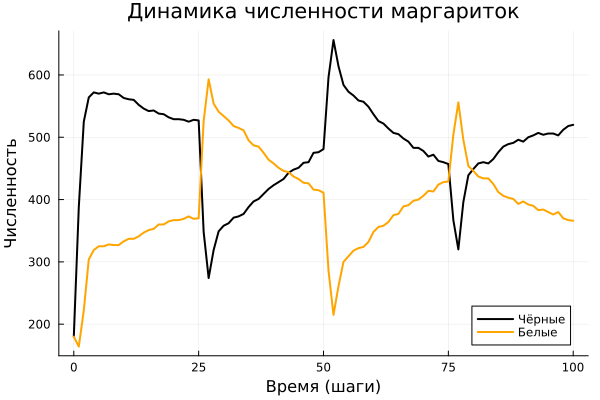
\includegraphics[width=0.55\linewidth,height=\textheight,keepaspectratio]{../report/image/daisyworld_count.png}
\end{frame}

\section{Полная динамика
(ramp)}\label{ux43fux43eux43bux43dux430ux44f-ux434ux438ux43dux430ux43cux438ux43aux430-ramp}

\begin{frame}{Трёхпанельный график динамики}
\phantomsection\label{ux442ux440ux451ux445ux43fux430ux43dux435ux43bux44cux43dux44bux439-ux433ux440ux430ux444ux438ux43a-ux434ux438ux43dux430ux43cux438ux43aux438}
Численность, температура, светимость

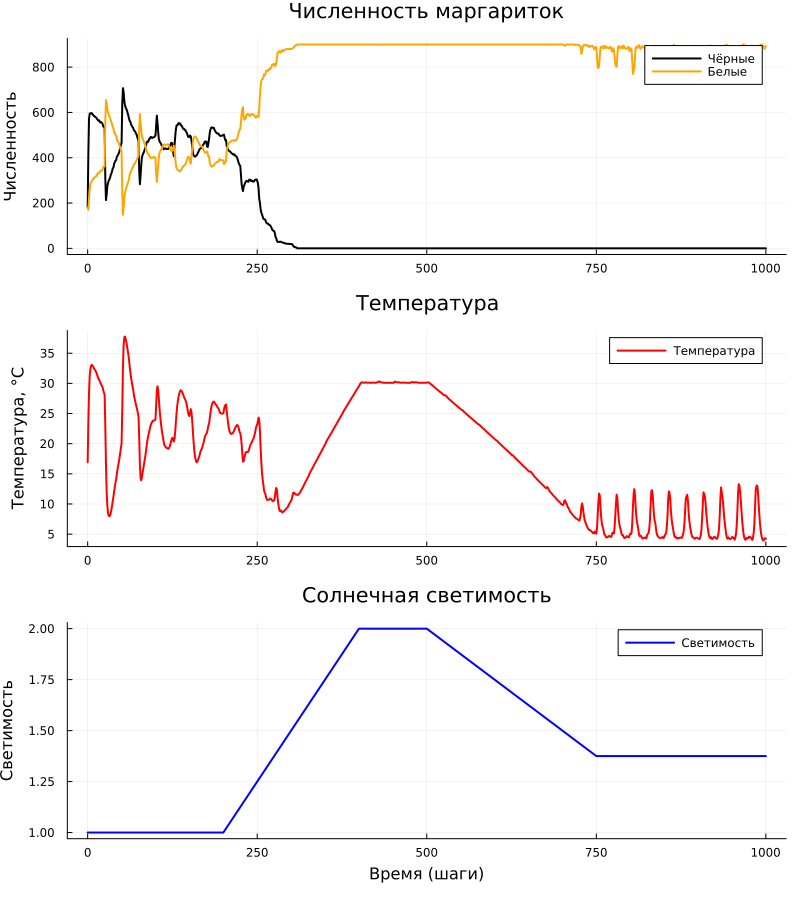
\includegraphics[width=0.45\linewidth,height=\textheight,keepaspectratio]{../report/image/daisyworld_luminosity.png}
\end{frame}

\section{Визуализация с
параметрами}\label{ux432ux438ux437ux443ux430ux43bux438ux437ux430ux446ux438ux44f-ux441-ux43fux430ux440ux430ux43cux435ux442ux440ux430ux43cux438}

\begin{frame}{Запуск daisyworld\_\_param.jl}
\phantomsection\label{ux437ux430ux43fux443ux441ux43a-daisyworld__param.jl}
Варьируем: init\_white (0.2, 0.8) и max\_age (25, 40) --- 4 комбинации

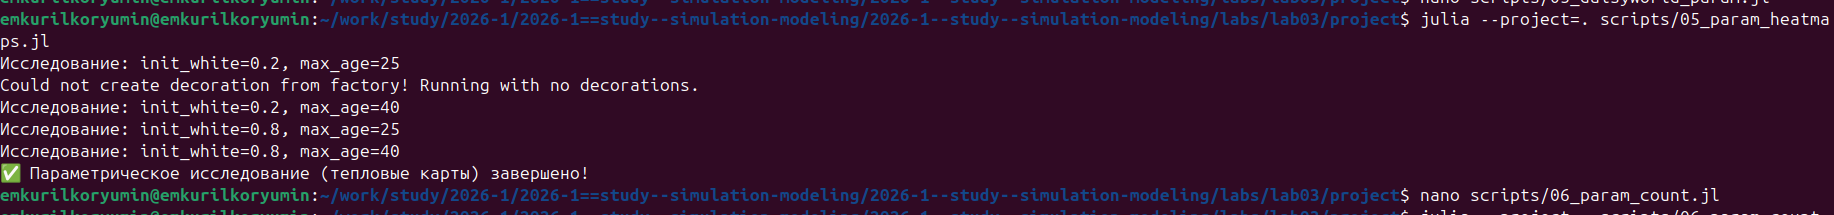
\includegraphics[width=0.55\linewidth,height=\textheight,keepaspectratio]{../report/image/04.png}
\end{frame}

\begin{frame}{init\_white=0.2, max\_age=25: шаг 0}
\phantomsection\label{init_white0.2-max_age25-ux448ux430ux433-0}
Начальное состояние: равные доли чёрных и белых

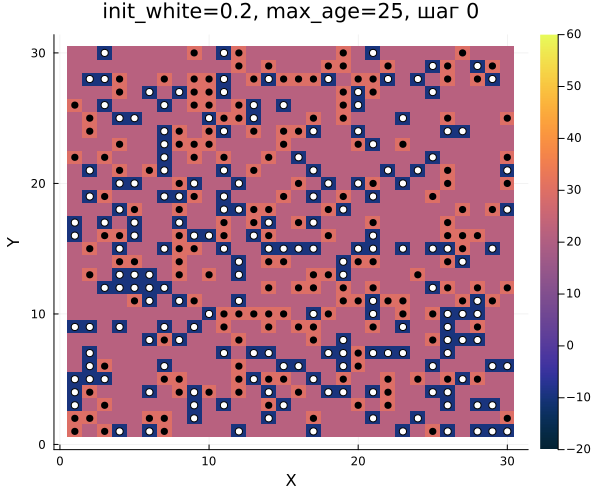
\includegraphics[width=0.45\linewidth,height=\textheight,keepaspectratio]{../report/image/daisyworld_iw0.2_ma25_step00.png}
\end{frame}

\begin{frame}{init\_white=0.2, max\_age=25: шаг 5}
\phantomsection\label{init_white0.2-max_age25-ux448ux430ux433-5}
Маргаритки начинают образовывать кластеры

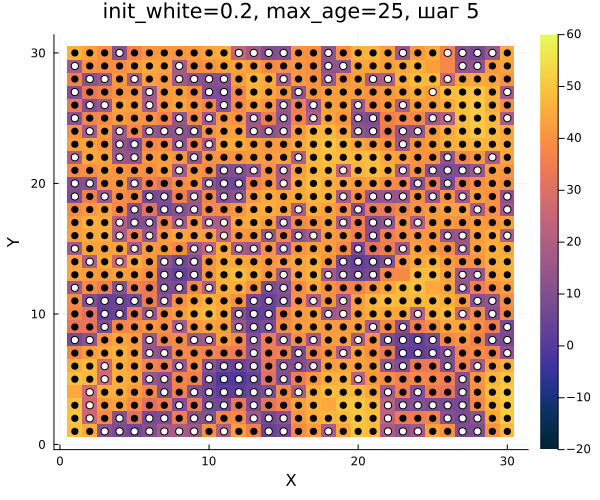
\includegraphics[width=0.45\linewidth,height=\textheight,keepaspectratio]{../report/image/daisyworld_iw0.2_ma25_step05.png}
\end{frame}

\begin{frame}{init\_white=0.2, max\_age=25: шаг 40}
\phantomsection\label{init_white0.2-max_age25-ux448ux430ux433-40}
Базовый случай: равномерное распределение обоих видов

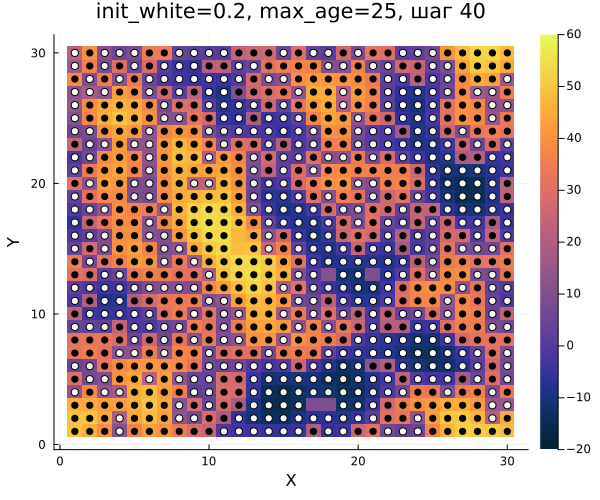
\includegraphics[width=0.45\linewidth,height=\textheight,keepaspectratio]{../report/image/daisyworld_iw0.2_ma25_step40.png}
\end{frame}

\begin{frame}{init\_white=0.2, max\_age=40: шаг 0}
\phantomsection\label{init_white0.2-max_age40-ux448ux430ux433-0}
Начальное состояние (увеличенный возраст)

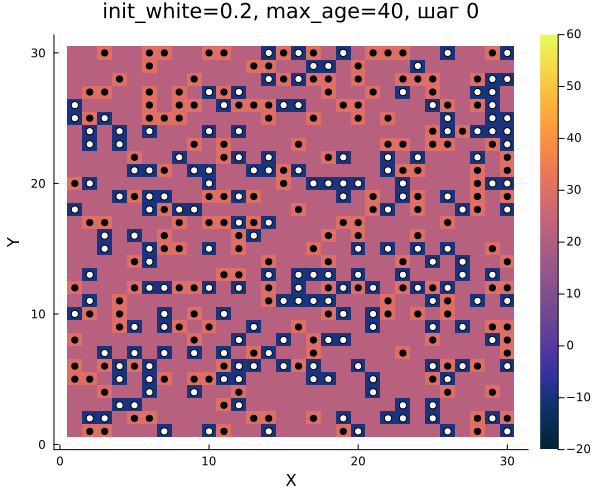
\includegraphics[width=0.45\linewidth,height=\textheight,keepaspectratio]{../report/image/daisyworld_iw0.2_ma40_step00.png}
\end{frame}

\begin{frame}{init\_white=0.2, max\_age=40: шаг 5}
\phantomsection\label{init_white0.2-max_age40-ux448ux430ux433-5}
Кластеры формируются быстрее

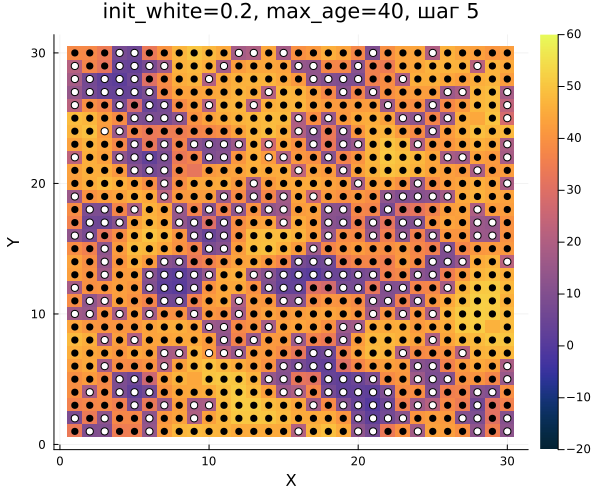
\includegraphics[width=0.45\linewidth,height=\textheight,keepaspectratio]{../report/image/daisyworld_iw0.2_ma40_step05.png}
\end{frame}

\begin{frame}{init\_white=0.2, max\_age=40: шаг 40}
\phantomsection\label{init_white0.2-max_age40-ux448ux430ux433-40}
Более плотное заполнение: маргаритки живут дольше

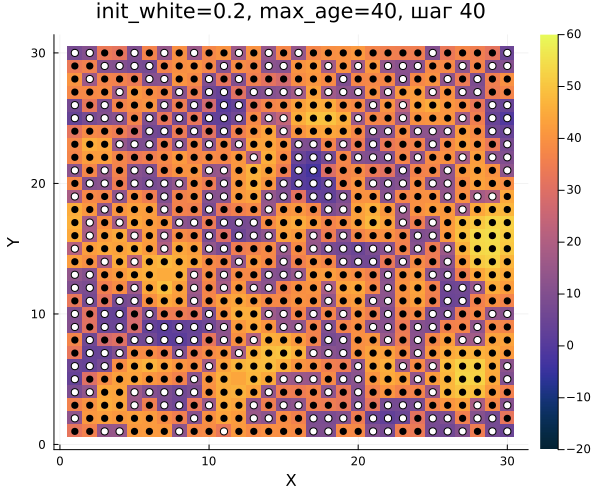
\includegraphics[width=0.45\linewidth,height=\textheight,keepaspectratio]{../report/image/daisyworld_iw0.2_ma40_step40.png}
\end{frame}

\begin{frame}{init\_white=0.8, max\_age=25: шаг 0}
\phantomsection\label{init_white0.8-max_age25-ux448ux430ux433-0}
80\% белых маргариток --- поверхность охлаждена

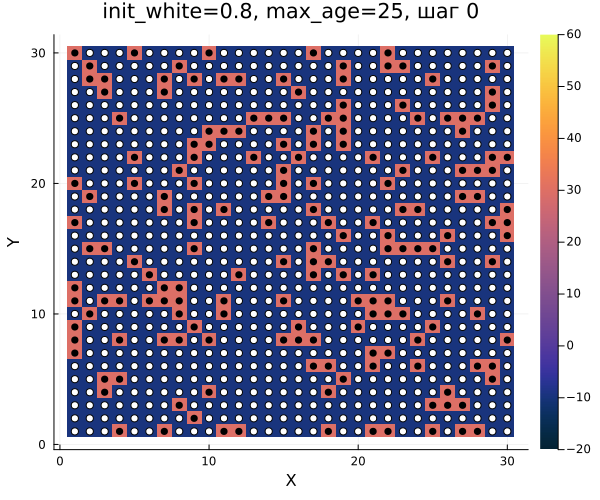
\includegraphics[width=0.45\linewidth,height=\textheight,keepaspectratio]{../report/image/daisyworld_iw0.8_ma25_step00.png}
\end{frame}

\begin{frame}{init\_white=0.8, max\_age=25: шаг 5}
\phantomsection\label{init_white0.8-max_age25-ux448ux430ux433-5}
Чёрные маргаритки начинают вытеснять белых

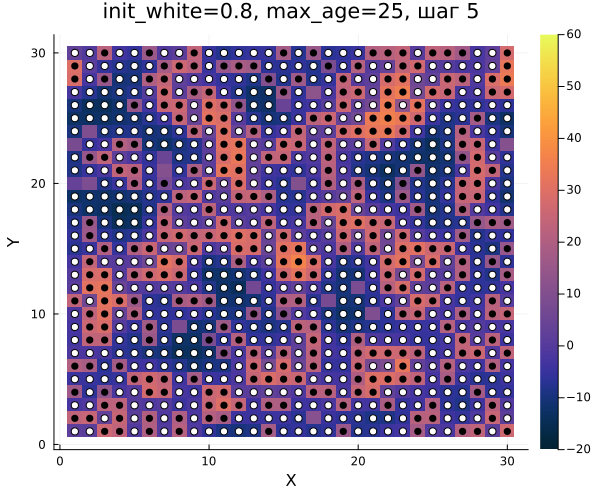
\includegraphics[width=0.45\linewidth,height=\textheight,keepaspectratio]{../report/image/daisyworld_iw0.8_ma25_step05.png}
\end{frame}

\begin{frame}{init\_white=0.8, max\_age=25: шаг 40}
\phantomsection\label{init_white0.8-max_age25-ux448ux430ux433-40}
Несмотря на 80\% белых вначале, равновесие то же

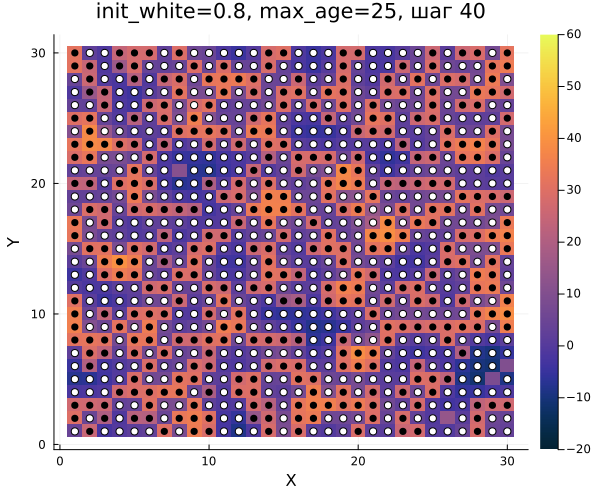
\includegraphics[width=0.45\linewidth,height=\textheight,keepaspectratio]{../report/image/daisyworld_iw0.8_ma25_step40.png}
\end{frame}

\begin{frame}{init\_white=0.8, max\_age=40: шаг 0}
\phantomsection\label{init_white0.8-max_age40-ux448ux430ux433-0}
Почти вся решётка --- белые маргаритки

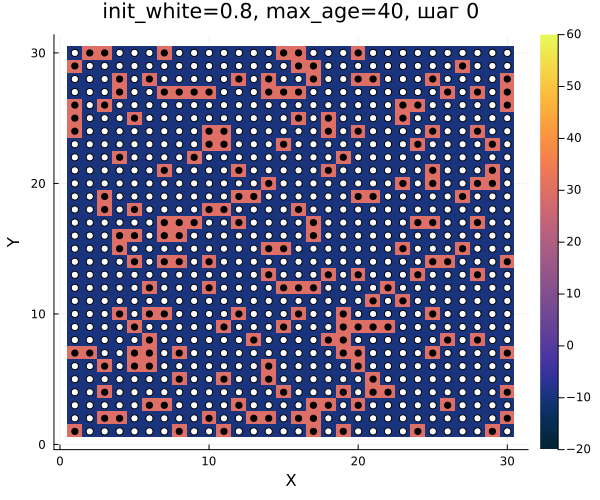
\includegraphics[width=0.45\linewidth,height=\textheight,keepaspectratio]{../report/image/daisyworld_iw0.8_ma40_step00.png}
\end{frame}

\begin{frame}{init\_white=0.8, max\_age=40: шаг 5}
\phantomsection\label{init_white0.8-max_age40-ux448ux430ux433-5}
Белые дольше преобладают из-за длинного жизненного цикла

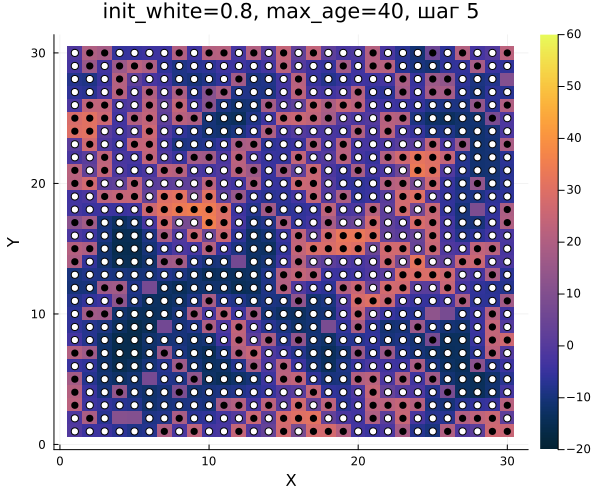
\includegraphics[width=0.45\linewidth,height=\textheight,keepaspectratio]{../report/image/daisyworld_iw0.8_ma40_step05.png}
\end{frame}

\begin{frame}{init\_white=0.8, max\_age=40: шаг 40}
\phantomsection\label{init_white0.8-max_age40-ux448ux430ux433-40}
Самая медленная динамика перехода к равновесию

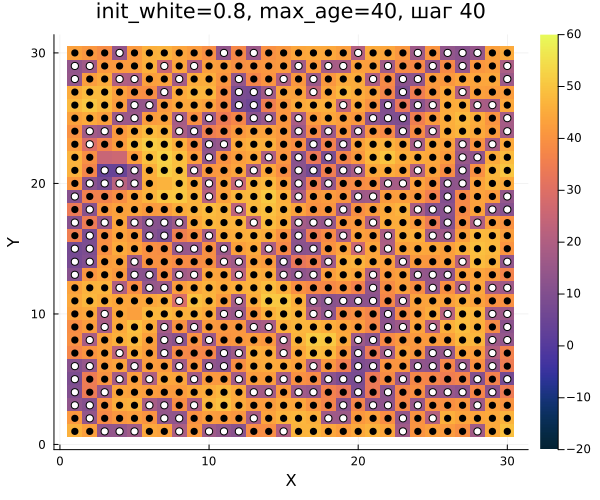
\includegraphics[width=0.45\linewidth,height=\textheight,keepaspectratio]{../report/image/daisyworld_iw0.8_ma40_step40.png}
\end{frame}

\section{Динамика с
параметрами}\label{ux434ux438ux43dux430ux43cux438ux43aux430-ux441-ux43fux430ux440ux430ux43cux435ux442ux440ux430ux43cux438}

\begin{frame}{Запуск daisyworld-count\_\_param.jl}
\phantomsection\label{ux437ux430ux43fux443ux441ux43a-daisyworld-count__param.jl}
Запуск скрипта динамики с параметрами

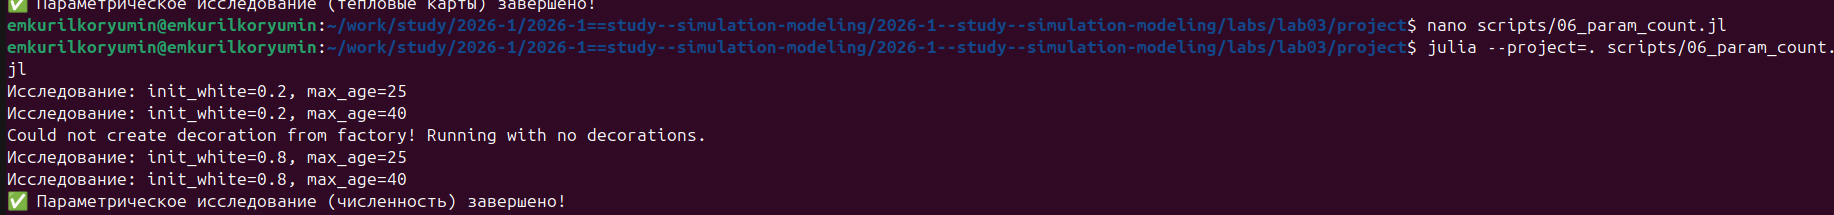
\includegraphics[width=0.6\linewidth,height=\textheight,keepaspectratio]{../report/image/05.png}
\end{frame}

\begin{frame}{init\_white=0.2, max\_age=25: динамика}
\phantomsection\label{init_white0.2-max_age25-ux434ux438ux43dux430ux43cux438ux43aux430}
Быстрые колебания, быстрое равновесие

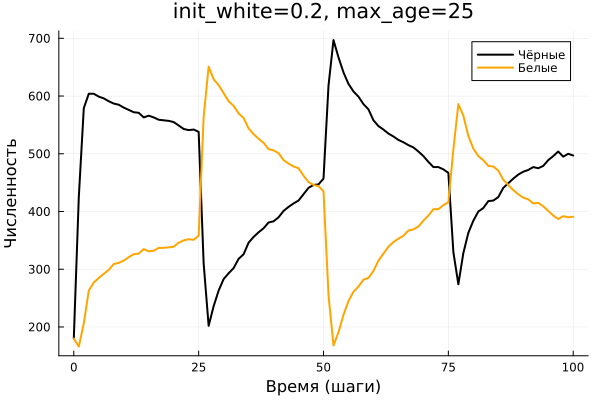
\includegraphics[width=0.5\linewidth,height=\textheight,keepaspectratio]{../report/image/daisy_count_iw0.2_ma25.png}
\end{frame}

\begin{frame}{init\_white=0.2, max\_age=40: динамика}
\phantomsection\label{init_white0.2-max_age40-ux434ux438ux43dux430ux43cux438ux43aux430}
Более плавная динамика

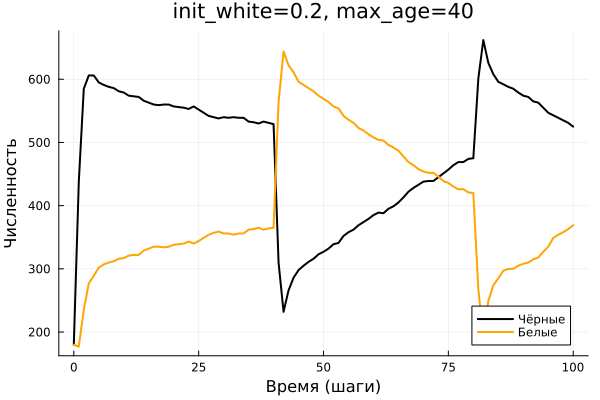
\includegraphics[width=0.5\linewidth,height=\textheight,keepaspectratio]{../report/image/daisy_count_iw0.2_ma40.png}
\end{frame}

\begin{frame}{init\_white=0.8, max\_age=25: динамика}
\phantomsection\label{init_white0.8-max_age25-ux434ux438ux43dux430ux43cux438ux43aux430}
Белые стартуют с 80\%, но равновесие то же

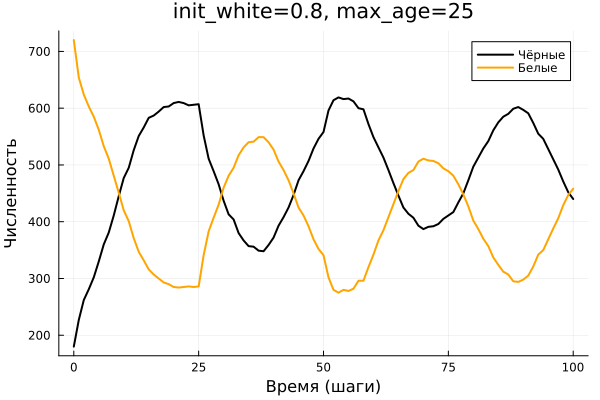
\includegraphics[width=0.5\linewidth,height=\textheight,keepaspectratio]{../report/image/daisy_count_iw0.8_ma25.png}
\end{frame}

\begin{frame}{init\_white=0.8, max\_age=40: динамика}
\phantomsection\label{init_white0.8-max_age40-ux434ux438ux43dux430ux43cux438ux43aux430}
Самый медленный переход к равновесию

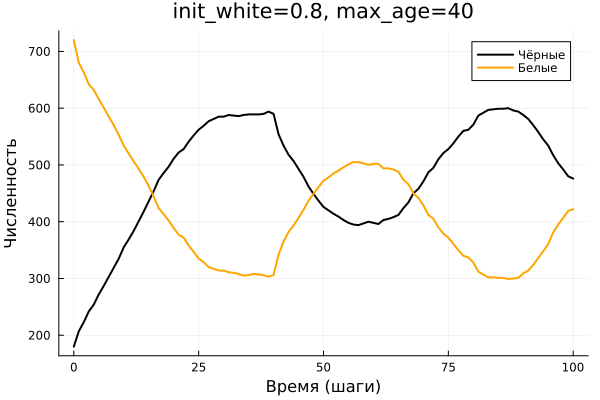
\includegraphics[width=0.5\linewidth,height=\textheight,keepaspectratio]{../report/image/daisy_count_iw0.8_ma40.png}
\end{frame}

\section{Полная динамика с параметрами
(ramp)}\label{ux43fux43eux43bux43dux430ux44f-ux434ux438ux43dux430ux43cux438ux43aux430-ux441-ux43fux430ux440ux430ux43cux435ux442ux440ux430ux43cux438-ramp}

\begin{frame}{Запуск daisyworld-luminosity\_\_param.jl}
\phantomsection\label{ux437ux430ux43fux443ux441ux43a-daisyworld-luminosity__param.jl}
Запуск скрипта полной динамики с параметрами

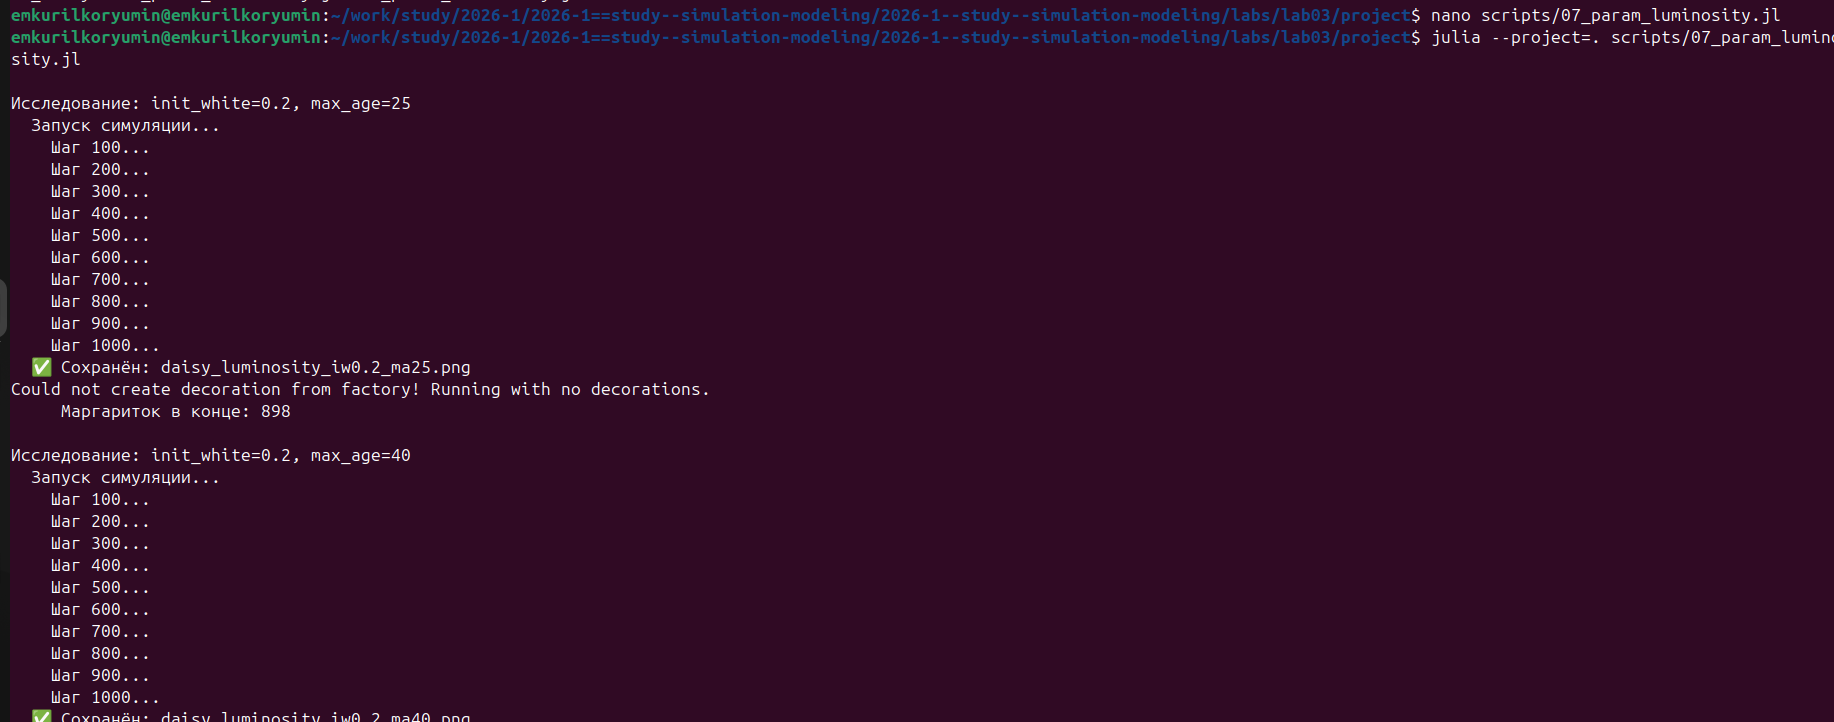
\includegraphics[width=0.6\linewidth,height=\textheight,keepaspectratio]{../report/image/06.png}
\end{frame}

\begin{frame}{init\_white=0.2, max\_age=25 (ramp)}
\phantomsection\label{init_white0.2-max_age25-ramp}
Быстрая адаптация к изменениям светимости

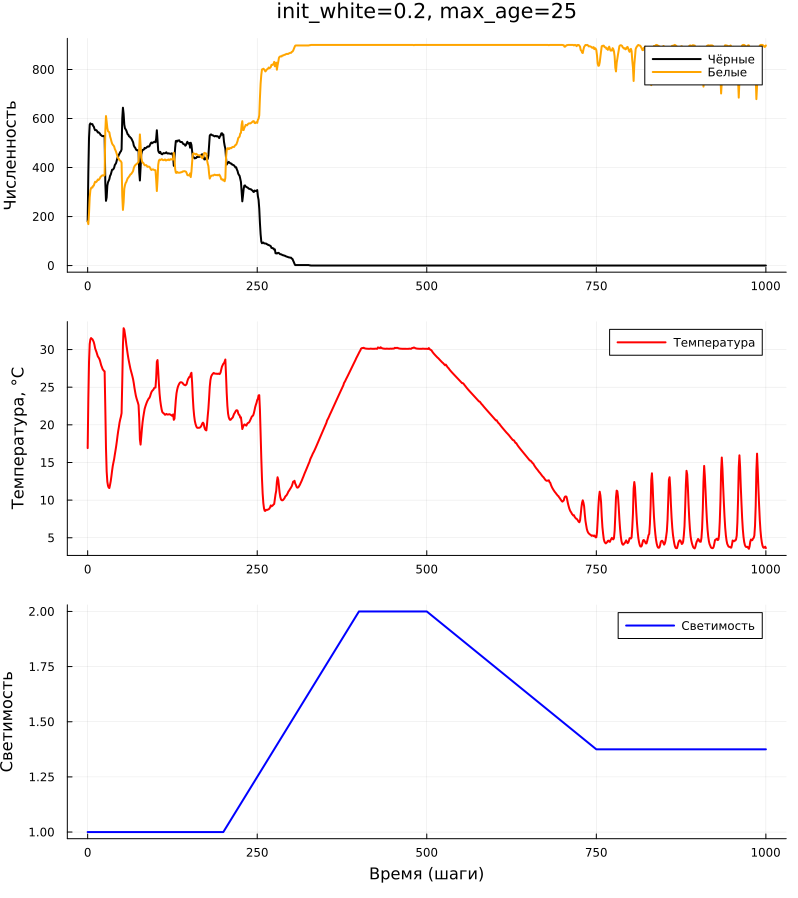
\includegraphics[width=0.45\linewidth,height=\textheight,keepaspectratio]{../report/image/daisy_luminosity_iw0.2_ma25.png}
\end{frame}

\begin{frame}{init\_white=0.2, max\_age=40 (ramp)}
\phantomsection\label{init_white0.2-max_age40-ramp}
Замедленная реакция, большая инерционность

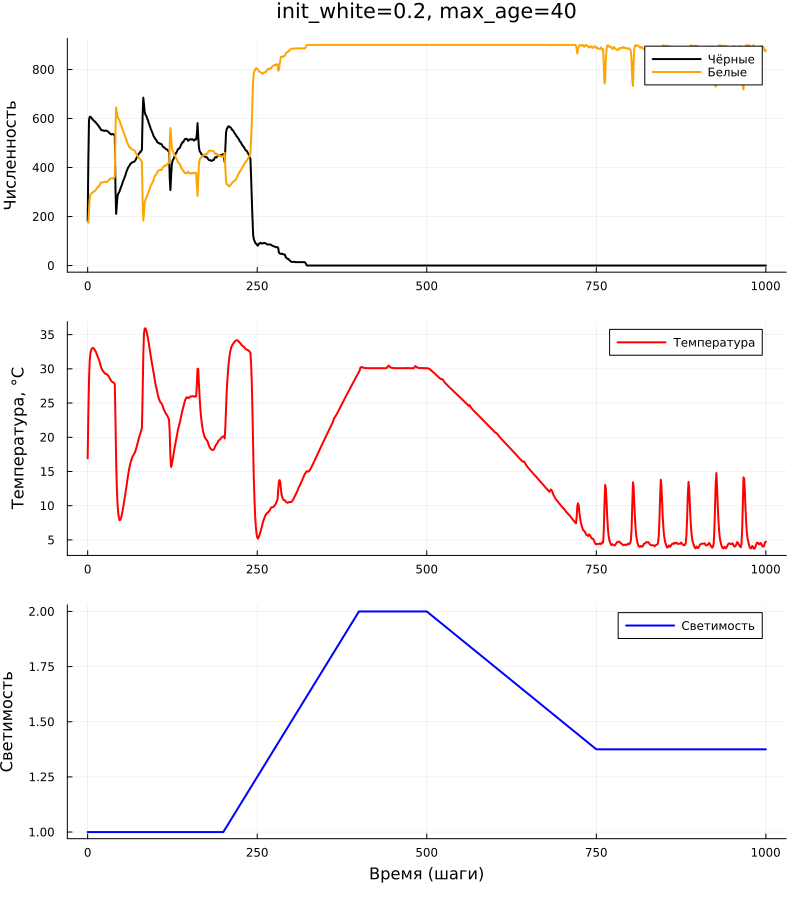
\includegraphics[width=0.45\linewidth,height=\textheight,keepaspectratio]{../report/image/daisy_luminosity_iw0.2_ma40.png}
\end{frame}

\begin{frame}{init\_white=0.8, max\_age=25 (ramp)}
\phantomsection\label{init_white0.8-max_age25-ramp}
Быстро забывает начальные условия

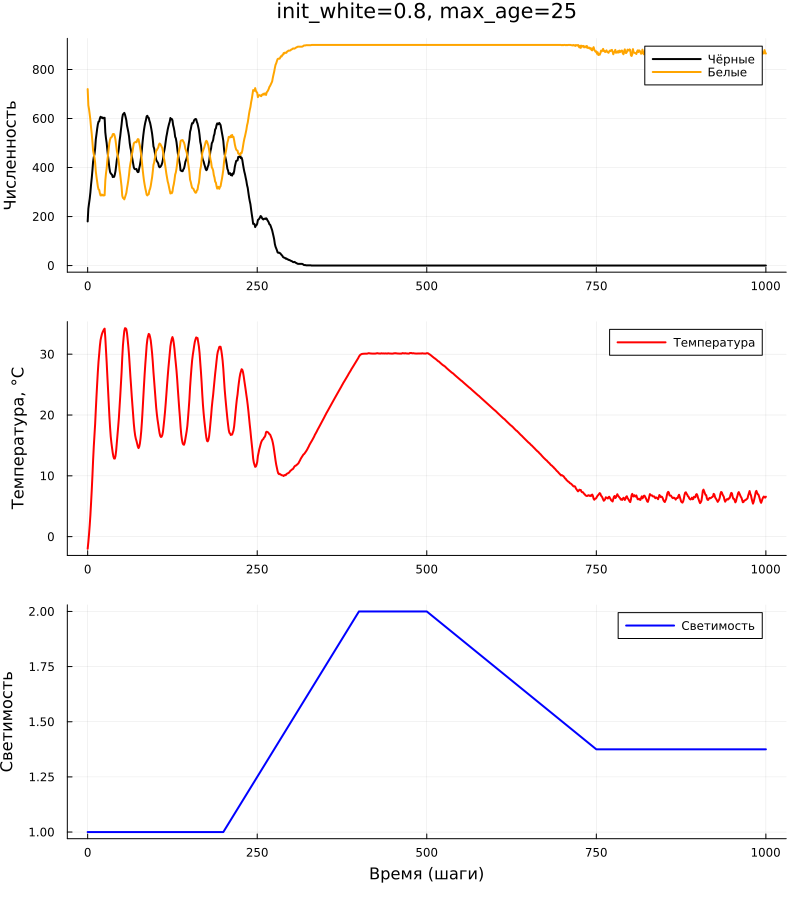
\includegraphics[width=0.45\linewidth,height=\textheight,keepaspectratio]{../report/image/daisy_luminosity_iw0.8_ma25.png}
\end{frame}

\begin{frame}{init\_white=0.8, max\_age=40 (ramp)}
\phantomsection\label{init_white0.8-max_age40-ramp}
Наиболее инерционная динамика

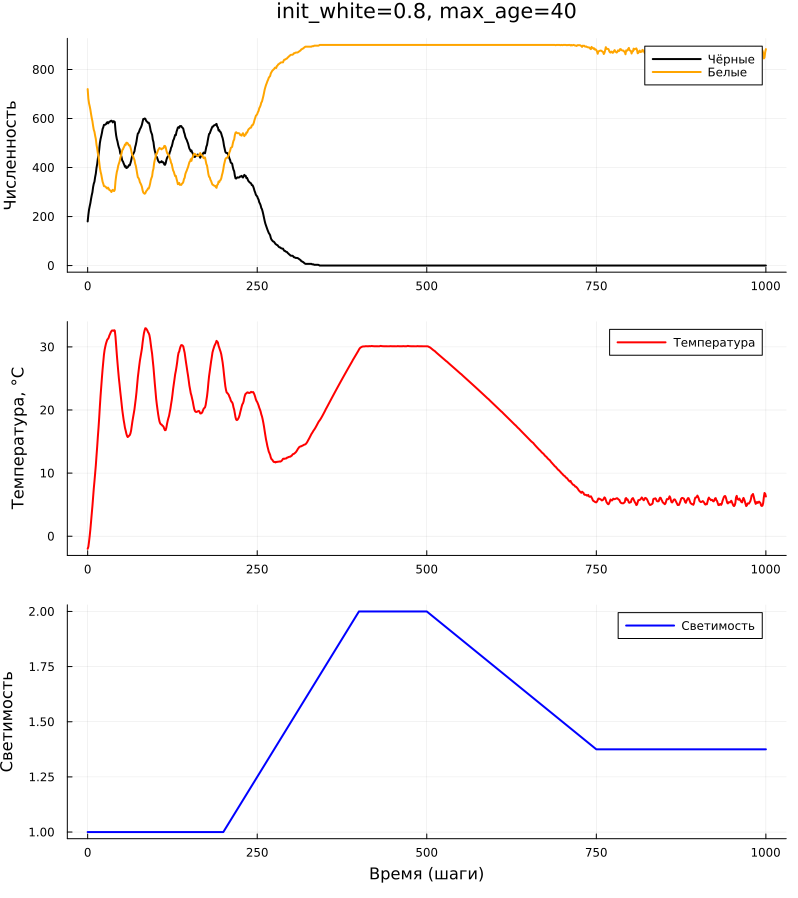
\includegraphics[width=0.45\linewidth,height=\textheight,keepaspectratio]{../report/image/daisy_luminosity_iw0.8_ma40.png}
\end{frame}

\section{Результаты}\label{ux440ux435ux437ux443ux43bux44cux442ux430ux442ux44b}

\begin{frame}[fragile]{Выводы}
\phantomsection\label{ux432ux44bux432ux43eux434ux44b}
\begin{itemize}
\tightlist
\item
  Реализована модель Daisyworld на Julia (Agents.jl)
\item
  Модель демонстрирует \textbf{эмерджентную саморегуляцию}
\item
  \texttt{init\_white}: влияет на переходную фазу, не на равновесие
\item
  \texttt{max\_age}: увеличивает плотность и инерционность
\item
  Сценарий ramp: маргаритки компенсируют изменения
\item
  6 скриптов, 18 производных файлов (Literate.jl)
\end{itemize}

:::
\end{frame}




\end{document}
